\chapter{Energy Calibration of the AHCAL}
\label{chap:ECalibAHCAL}

The CALICE Analog Hadronic Calorimeter (AHCAL) technological prototype was installed at the SPS CERN facilities in July and August 2015, in order to provide energy and time measurements of electromagnetic and hadronic showers using plastic scintillators. The data recorded in each cells of the calorimeter is measured in ADC counts, thus this scale cannot be compared directly between different channels. Therefore to compare them, all channels have to be scaled to a common physical energy unit. For the AHCAL, the Minimum Ionizing Particle or MIP unit is chosen. This unit relates to the cell energy in a well and understood physical process almost independent to outside conditions.

The conversion requires a calibration of each cells of the calorimeter which is by itself a challenge due to the high number of readout channels. In this testbeam, 3744 channels have to be calibrated. Due to the boards equipped with SiPMs from various different batches, the procedure needs to be automatic and robust to extract the calibration constant for each channel. At the end, all the calibration constants are entered in the official CALICE database.

This chapter will firstly describe the beamline facilities used in July 2015 at CERN, followed by the description of the tesbeam setup and finally describe the procedure performed for the AHCAL energy calibration.

\section{Beamline Setup}

During the summer of 2015, CALICE performed several testbeam campaigns with the AHCAL technological prototype. The detector was installed in the beamline H2 at the North Area beamline at CERN \cite{H2Beamline}. The beamline provided wire chambers and scintillators that enabled us to have informations about the beam position and number of particles but unfortunately no data from theses detectors were recorded. Few information was collected about the amount of material upstream of the detector until the last momentum selection magnet. A Cherenkov detector (at around 500 m upstream) was also available to tag incoming particles. These detectors make advantage of the fact, a particle that traverses a medium faster than the speed of light in that medium will generate a cone of cherenkov light \cite{}. This light can then be collected by a photomultiplier. The detector at this beamline offered the possiblity to set a threshold for particle tagging. Usually, the threshold is set to distinguish between electrons and pions/kaons. This is particularly needed to tag electrons in pion runs. The tagging signal provided by the Cherenkov detector was fed to several AHCAL channels in order to be able to tag events.\\

For the production of particles, a primary high intensity proton beam (around $10^{12}$ protons per burst) of 400 GeV is impinged on a target. From this a secondary beam is produced containing various particles type and energies. For muons, the beam is obtained by scrapping the halo of a pion beam with collimators. For electrons, a neutral beam of photons is send to a lead target to generate electrons from gamma conversion, producing a very pure electron beam. For pions, the beam is selected via a set of collimators and magnets. Due to the decay of $\pi_0$ and the acceptance of the beamline, a contamination of the pion beam with electrons is possible at low momentum (< 20 GeV).

\section{TestBeam Setup}

In July 2015, the AHCAL detector was using the full EUDET steel stack \cite{EUDET-Report-2010-02} with 48 iron absorber plates. Of it, 14 layers of active material was available for this testbeam as shown in figures \ref{fig:Det_layout} and \ref{fig:AHCAL_photo}. The data was recorded with beam from 10 to 90 GeV. The detector was placed on a movable stage, in order to be able to move the detector relative to the beam for muon calibration runs. This thesis will analyse muon data, electron showers between 10 and 50 GeV and pion showers between 10 and 90 GeV focusing on the timing aspect of the detector.

\begin{figure}[htbp!]
	\centering
	\includegraphics[width=1\linewidth]{chap5/fig_EnergyCalib/Detector_layout.png}
	\caption{Simplified view of the detector layout.} \label{fig:Det_layout}
\end{figure}

The beam instrumentation was consisted of two $10 \times 10$ cm$^2$ (in front of the calorimeter) as well as two $50 \times 50$ cm$^2$ (in front and back) scintillator plates readout with photomultiplier tubes. The coincidence of the $50 \times 50$ cm$^2$ scintillator was used for the muon runs and the coincidence of the $10 \times 10$ cm$^2$ scintillator was used for the electron and pion runs. Additionally, the coincidence signal from the scintillator was fed to several channels in the AHCAL in order to provide a reference time for the trigger which is important in this analysis.

\begin{figure}[htbp!]
	\centering
	\includegraphics[width=0.8\linewidth]{chap5/fig_EnergyCalib/IMG_1170.jpg}
	\caption{Photo of the AHCAL detector before the installation in the testbeam area.} \label{fig:AHCAL_photo}
\end{figure}

\section{Energy Calibration of the AHCAL}

Every channel of the detector provides a measure of the energy deposited in ADC units. To compare them or combined them, all channels need to be normalized to a common physics scale. The AHCAL uses muons to provide the calibration to the common scale as Minimum Ionizing Particles or MIP. Therefore muon runs were recorded. As detailled in section \ref{}, the energy deposited in a single AHCAL cell follows approximatively a Landau distribution but due to the electronic noise, the resulting response is convoluted with a Gaussian distribution. The MPV of the Laudau-Gaussian convoluted function is defined as the MIP constant (ADC$_{MIP_i}$) for the i-th channel.

\subsection{Pedestal extraction}

To obtain the correct MIP constant, a pedestal substraction has to be done. The pedestal value for each channels is extracted from the data taking muon runs. In order to be consistant, the pedestal value is extracted in the same running mode as data taking .i.e in auto-trigger (AT). For each channel and memory cell, an histogram is filled with the ADC value of a cycle in case no Hit Bit is set for the channel. The extraction is performed in an iterative way due to a high tail in energy that is not yet understood.

\begin{figure}[htbp!]
	\centering
	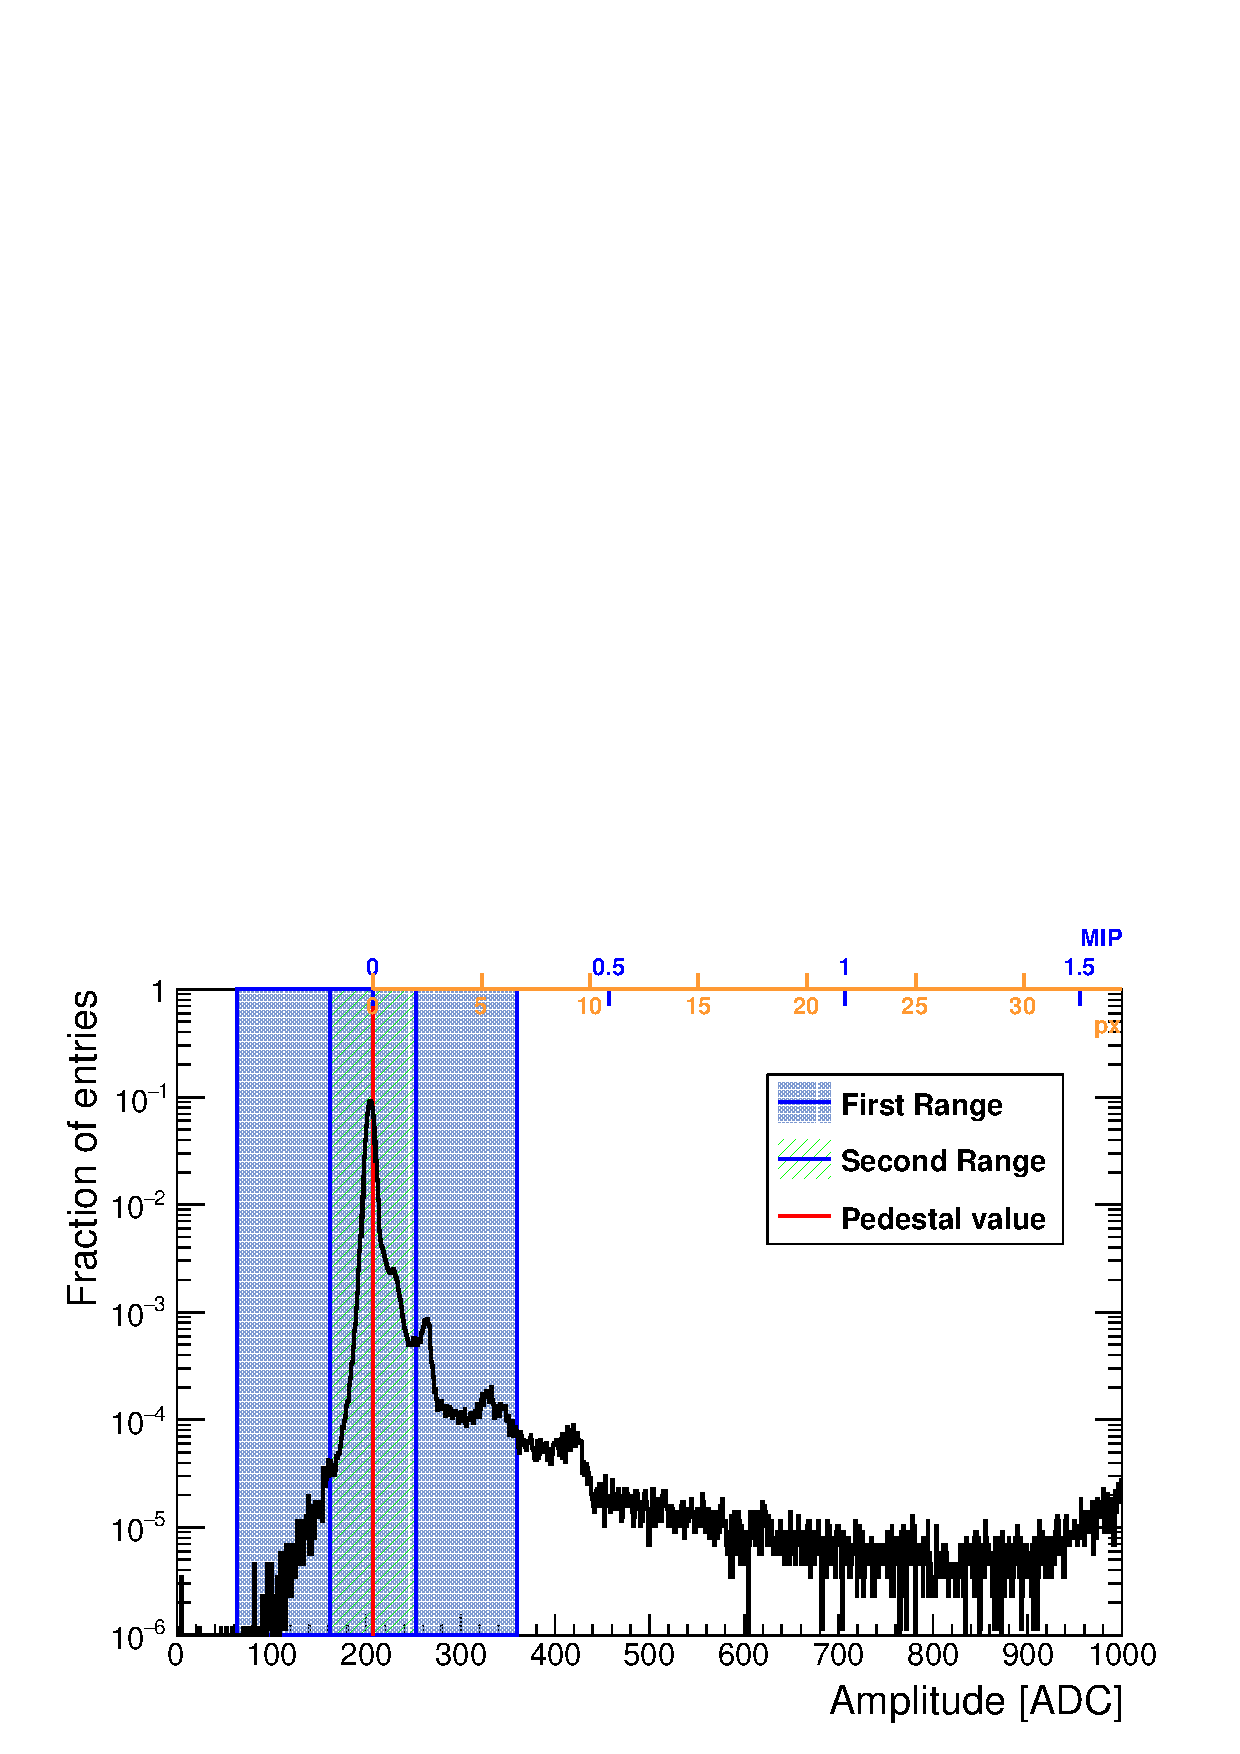
\includegraphics[width=0.8\linewidth]{chap5/fig_EnergyCalib/PedestalExtractionExample.pdf}
	\caption{Typical pedestal distribution of a channel in auto-trigger mode. The different colored boxed represent the iterative procedure to extract the pedestal value marked with the red line.} \label{fig:PedExtraction}
\end{figure}

As the SiPM noise needs to be taken into account for the pedestal value and considering a poisson statistic, one to three pixels could be fired due to DCR and cross-talk. The fitting range then needs to be in the same order of magnitude of 1 to 3 pixels. For this, the histogram is reduced in the range of 3 RMS around the mean 2 times. After the mean of the histogram is taken the pedestal value as shown in figure \ref{fig:PedExtraction}. As no pedestal substraction memory cell-wise is performed in the reconstruction at the moment and the database structure is not designed to have the pedestal constant for each memory cell, a mean over all memory cell is computed per channel. The average difference between the mean pedestal and the memory cell wise pedestal shown in figure \ref{fig:CompMeanMem} is around 21 ADC which would correspond to an error of about 4\% on the MIP constant (assuming a MIP value of 500 ADC). This error is dominating in the MIP constant uncertainty.

\begin{figure}[htbp!]
	\centering
	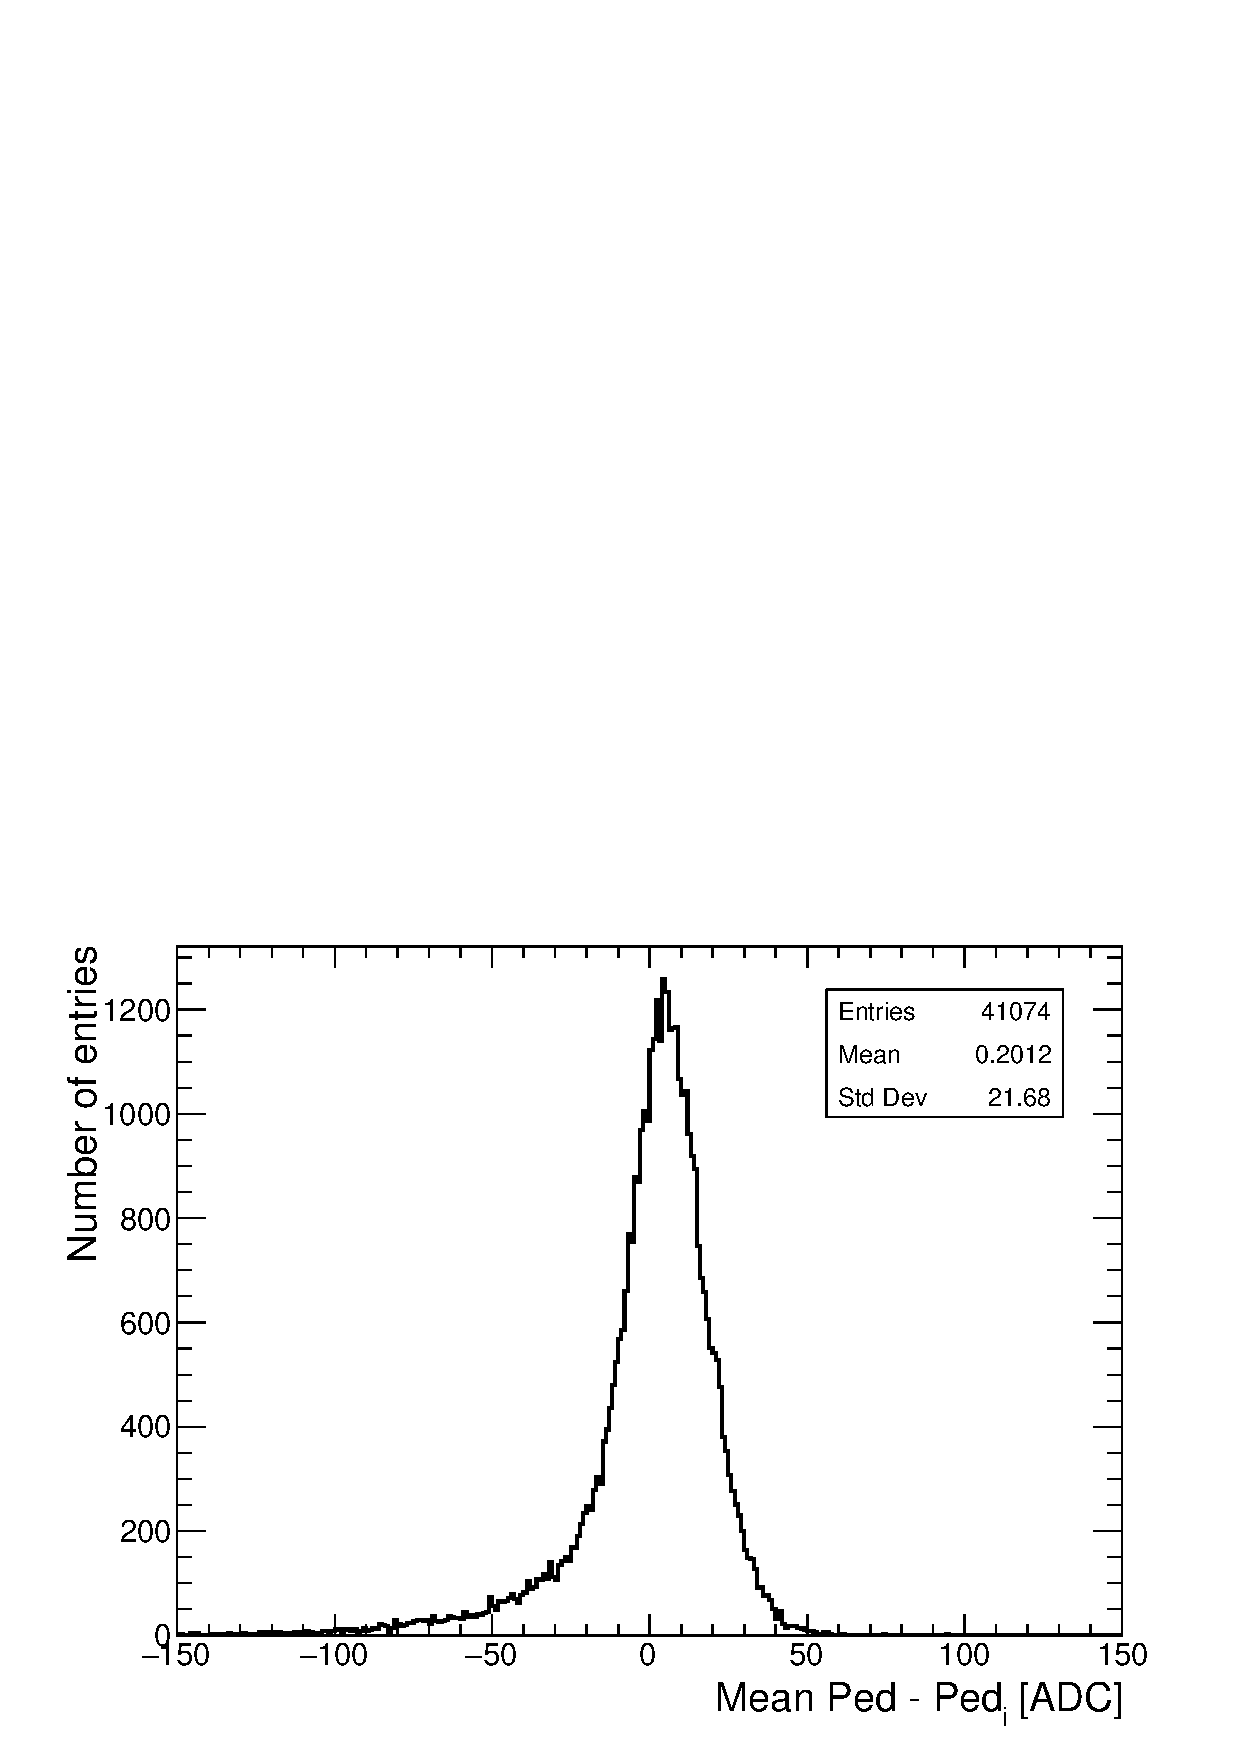
\includegraphics[width=0.8\linewidth]{chap5/fig_EnergyCalib/ComparisonMeanPedtoMemorycell.pdf}
	\caption{Distribution of the difference between the mean pedestal to the memory-cell wise pedestal per channel.} \label{fig:CompMeanMem}
\end{figure}

\subsection{MIP extraction}

After the pedestal calibration, the extraction of the MIP constant for each channel can be performed. As the detector was equipped with various types of SiPM and boards designs, the extraction procedure needed to be automatised and robust. In order to reduce noise in the energy spectra of each cell that would lead to unstable fits and wrong MIP constants, a simple tracking selection has been performed as explained in section \ref{subsec:Muon_sel}.
